% 范畴论
% 范畴|元素|同构|群胚|函子|Yoneda

\subsection{基本概念}
\begin{definition}{范畴}
\textbf{范畴} $\mathcal{C}$ 包含以下结构.
\begin{enumerate}
    \item 存在一类\textbf{元素} $\operatorname{Ob}(\mathcal{C})$;
    \item 对于每对元素 $X,Y\in\operatorname{Ob}(\mathcal{C})$,存在一类\textbf{态射} $\operatorname{Mor}_\mathcal{C}(X,Y)$;
    \item 对于每三个元素 $x,y,z\in\operatorname{Ob}(\mathcal{C})$,存在态射复合映射 ${\circ}:\operatorname{Mor}_\mathcal{C}(Y,Z)\times\operatorname{Mor}_{\mathcal{C}}(X,Y)\to\operatorname{Mor}_\mathcal{C}(X,Z)$.
\end{enumerate}
这些结构满足以下规则.
\begin{enumerate}
    \item 对于每个元素 $X\in\operatorname{Ob}(\mathcal{C})$,存在\textbf{单位态射} $\operatorname{id}_X\in\operatorname{Mor}_\mathcal{C}(X,X)$,使得 $\operatorname{id}_X\circ\phi=\phi$ 和 $\psi\circ\operatorname{id}_X=\psi$ 成立,其中 $\phi\in\operatorname{Mor}_\mathcal{C}(Y,X)$ 对于任意 $Y\in\operatorname{Ob}(\mathcal{C})$, $\psi\in\operatorname{Mor}_\mathcal{C}(X,Z)$ 对于任意 $Z\in\operatorname{Ob}(\mathcal{C})$;
    \item 复合具有结合性,即对于 $\phi\in\operatorname{Mor}_\mathcal{C}(Y,Z),\psi\in\operatorname{Mor}_\mathcal{C}(X,Y),\chi\in\operatorname{Mor}_\mathcal{C}(W,X)$,有 $(\phi\circ\psi)\circ\chi=\phi\circ(\psi\circ\chi)$;
    \item 任意态射集合 $\opn{Mor}_\mathcal{C}(X,Y)$ 和 $\opn{Mor}_\mathcal{C}(X',Y')$ 不交,除非 $X=X',Y=Y'$,此时它们相等.
\end{enumerate}
\end{definition}
由于以下练习,我们讨论单位态射的时候可以省去选择,只讨论唯一的单位映射.
\begin{exercise}{}
证明同个元素的任意两个单位态射是相等的.
\end{exercise}
有时我们也会使用 $\operatorname{dom}$ (\textbf{域})和 $\operatorname{cod}$ (\textbf{陪域})来讨论态射.值得注意的是,我们一般情况下要求元素为一个集合而不是一个类,仅在如下范畴中我们放宽要求允许元素为一个真类:
\begin{itemize}
    \item 集合范畴 $(\mathbf{Set})$,态射为映射;
    \item 交换群范畴 $(\mathbf{Ab})$,态射为交换群同态;
    \item 群范畴 $(\mathbf{Grp})$,态射为群同态;
    \item 左 $G$-群作用范畴 $(\mathbf{G{-}Set})$,态射为 $G$-映射;
    \item 对于含幺交换环 $R$,模范畴 $(\mathbf{R{-}Mod})$,态射为模同态;
    \item 对于域 $F$,向量空间范畴 $(\mathbf{F{-}Vect})$,态射为线性映射;
    \item 拓扑空间范畴 $(\mathbf{Top})$,态射为连续映射;
    \item 含幺交换环范畴 $(\mathbf{Ring})$,态射为环同态.
\end{itemize}
我们称 $\opn{Ob}$ 为一集合的范畴\textbf{集合范畴},称其为\textbf{真类范畴}若其 $\opn{Ob}$ 不构成集合.另外,若一真类范畴的每个态射类都构成集合,我们称它是一个\textbf{局部集合范畴}.
为简化我们所使用的符号,若所讨论的范畴在上下文中没有歧义,可使用符号 $\opn{Ob}$ 和 $\opn{Mor}(X,Y)$;另对于态射 $\phi\in\opn{Mor}(X,Y)$,我们通常使用映射符号将其写为 $\phi:X\to Y$.

\begin{definition}{范畴论同构}
对于一个态射 $\phi:X\to Y$,若存在另一个态射 $\psi:Y\to X$ 使得 $\phi\circ\psi=\opn{id}_Y$ 和 $\psi\circ\phi=\opn{id}_X$ 成立,则我们说它是一个范畴论同构.此时 $\phi$ 也被称为一个可逆态射,而 $\phi^{-1}=\psi$ 则被称为它的逆.
\end{definition}
若一态射的域和陪域相同,则它可被称为一个\textbf{自态射},元素 $X\in\opn{Ob}$ 的所有自态射形成一个幺半群,被称为 $\opn{Endo}_\mathcal{C}(X)$;若它还是一个同态,则被称为\textbf{自同态},所有元素 $X$ 的自同态形成一个群,被称为 $\opn{Auto}_\mathcal{C}(X)$.

\begin{definition}{群胚}
若范畴 $\mathcal{C}$ 的所有态射都是范畴论同构,则称范畴 $\mathcal{C}$ 为一\textbf{群胚}.
\end{definition}
群胚是群的一般化结构.一个群 $G$ 可以生成一个群胚,使得其结构被保留:这个群胚由一个元素 $X$ 构成,其仅有的态射为 $\opn{Mor}(X,X)=G$,态射复合被定义为 $a\circ b=ab$,请自行验证如此定义的范畴为一个群胚.集合 $A$ 也可生成群胚,定义
\begin{equation}
\opn{Ob}=A\quad\opn{Mor}(X,Y)=\begin{cases}\emptyset&X\neq Y\\\{\opn{id}\}&X=Y\end{cases}
\end{equation}
请自行验证它是一个群胚.

\begin{definition}{函子}
范畴 $\mathcal{A},\mathcal{B}$ 间的\textbf{协变函子} $F:\mathcal{A}\to\mathcal{B}$ 包含以下结构.
\begin{enumerate}
    \item 若 $\mathcal{A}$ 和 $\mathcal{B}$ 均为集合范畴,则函子包含一个映射 $F_{\opn{Ob}}^{\text{Set}}:\opn{Ob}(\mathcal{A})\to\opn{Ob}(\mathcal{B})$,否则函子包含一个从 $\opn{Ob}(\mathcal{A})$ 到 $\opn{Ob}(\mathcal{B})$ 的\textbf{关联} $F_{\opn{Ob}}^{\text{PrCl}}$;
    \item 函子包含一个映射 $F_{\opn{Mor}}:\opn{Mor}_\mathcal{C}(X,Y)\to\opn{Mor}_\mathcal{B}(F_{\opn{Ob}}^{\text{Set/PrCl}}(X),F_{\opn{Ob}}^{\text{Set/PrCl}}(Y))$,对于每个 $x,y\in\opn{Ob}(A)$.
\end{enumerate}
函子满足如下公理.
\begin{enumerate}
    \item 对于任意元素 $X\in\opn{Ob}(A)$, $F(\opn{id}_X)=\opn{id}_{F(x)}$;
    \item 对于任意可复合的元素对 $(\phi,\psi)$, $F(\phi\circ_\mathcal{A}\psi)=F(\phi)\circ_\mathcal{B}F(\psi)$.
\end{enumerate}
\end{definition}
我们仅考虑域和陪域为上方列出的真类范畴的具有 $F_{\opn{Ob}}^{\text{PrCl}}$ 的函子.我们考虑的大部分范畴和函子都是\textbf{数学对象}(可用ZFC公理化集合论描述的对象).注意若函子对象关系的类型(映射或关联)明确,我们可以将其省略.另外我们也会在语义明确时省略下标 $\opn{Ob}$ 和 $\opn{Mor}$. 任何范畴 $\mathcal{A}$ 都有一个显然的单位函子 $\opn{id}_\mathcal{A}$, 同时对于两个函子 $F:\mathcal{A}\to\mathcal{B}$ 和 $G:\mathcal{B}\to\mathcal{C}$,我们可以定义它们的复合.

\textbf{TODO} opposite category and contravariant functor

\textbf{TODO} natural transformation

\subsection{$\opn{Hom}$函子和Yoneda引理}
\begin{definition}{$\opn{Hom}$函子}
若 $\mathcal{C}$ 是一个局部集合范畴,对于每个 $A\in\mathcal{C}$,记 $A$-协变 $\opn{Hom}$ 函子为 $h^A=\opn{Hom}(A,-):\mathcal{C}\to\mathbf{Set}$,其定义如下:
\begin{itemize}
\item 若 $X\in\opn{Ob}(\mathcal{C})$,则 $h^A(X)=\opn{Mor}_\mathcal{C}(A,X)\in\opn{Ob}(\mathbf{Set})$;
\item 若 $f\in\opn{Mor}_\mathcal{C}(X,Y)$,则对于 $g:A\to X$,有 $h^A(f)=g\mapsto f\circ g:A\to Y\in h^A(Y)$.
\end{itemize}

记 $B$-逆变 $\opn{Hom}$ 函子为 $h_B=\opn{Hom}(-,B):\mathcal{C}\to\mathbf{Set}$,其定义如下:
\begin{itemize}
\item 若 $X\in\opn{Ob}(\mathcal{C})$,则 $h_A(X)=\opn{Mor}_\mathcal{C}(X,B)\in\opn{Ob}(\mathbf{Set})$;
\item 若 $f\in\opn{Mor}_\mathcal{C}(X,Y)$,则对于 $g:X\to B$,有 $h_A(f)=g\mapsto g\circ f:Y\to B\in h_A(Y)$.
\end{itemize}
\end{definition}
若我们使用现代代数几何的语言,如上定义的逆变 $\opn{Hom}$ 函子还可被称为一个\textbf{预层}.
\begin{definition}{$\opn{Hom}$函子范畴}
我们使用$\mathbf{Set}^\mathcal{C}$来记协变 $\opn{Hom}$ 函子所构成的范畴,对于每个 $\mathcal{C}$ 中的态射 $\phi:A'\to A$,我们可以获得一个自然变换 $h_{\text{co}}(\phi):(h^A:\mathcal{C}\to\mathbf{Set})\Rightarrow(h^{A'}:\mathcal{C}\to\mathbf{Set})$.
我们可以简单地看出,下图是交换的对于任意 $\psi\in\opn{Mor}_\mathcal{C}(X,Y)$,于是 $h_\text{co}(\phi)$ 的确是一自然变换.
\begin{figure}[h!]
\centering
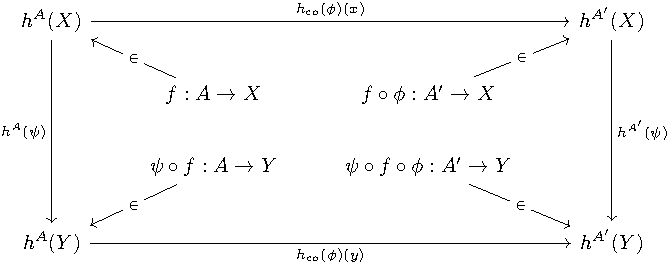
\includegraphics[width=13cm]{./figures/Cat1.pdf}
\caption{$h_{\text{co}}(\phi)$ 的自然性} \label{Cat_fig1}
\end{figure}
类似地,我们可以定义逆变 $\opn{Hom}$ 函子所构成的范畴 $\mathbf{Set}^{\mathcal{C}^\text{op}}$,唯一不同的一点是我们需要给出一个相反的映射 $\phi:B\to B'$来使得下图交换.注意下图中 $h_B(-)$是一逆变函子,所以关于图交换的结论是对于 $\psi:Y\to X$而言的.
\begin{figure}[ht]
\centering
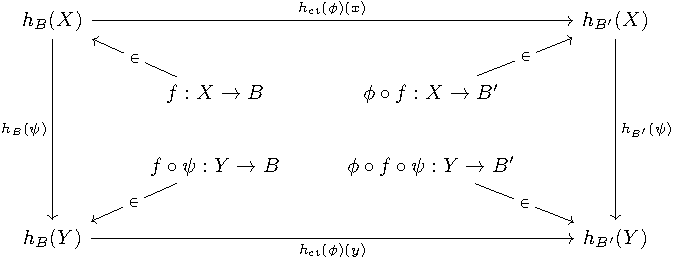
\includegraphics[width=13cm]{./figures/Cat2.pdf}
\caption{$h_{\text{ct}}(\phi)$的自然性} \label{Cat_fig2}
\end{figure}
\end{definition}
如上定义的 $\mathbf{Set}^{\mathcal{C}^\text{op}}$在代数几何中也被记为 $\mathbf{PSh}(\mathcal{C})$.
\begin{exercise}{}
请验证 $h^{-}:\mathcal{C}\to\mathbf{Set}^\mathcal{C}$和 $h_{-}:\mathcal{C}\to\mathbf{Set}^{\mathcal{C}^\text{op}}$为函子.提示:观察上述定义,可以注意到前者为逆变函子,后者为协变函子.
\end{exercise}

\begin{theorem}{Yoneda引理}
对于任意局部集合范畴 $\mathcal{C}$和 $A,B\in\opn{Ob}(\mathcal{C})$,
\begin{enumerate}
\item 给定协变函子 $F:\mathcal{C}\overset{\text{co}}{\to}\mathbf{Set}$,存在双射 $\opn{Nat}(h^A,F)\simeq F(A)$;
\item 给定逆变函子 $G:\mathcal{C}\overset{\text{ct}}{\to}\mathbf{Set}$,存在双射 $\opn{Nat}(h_B,G)\simeq G(B)$
\end{enumerate}
\end{theorem}
\textbf{证明.}
对于自然变换 $\Phi:h^A\Rightarrow F$,我们将它映射到 $u=m(\Psi)=\Phi_A(\opn{id}_A)$(注意此处 $\Phi_A$是 $\mathbf{Set}$中 $h^A(A)\to F(A)$的态射,即一个映射);对于 $v\in F(A)$,将它映射到如 $\Psi_X(f:\opn{Mor}_\mathcal{C}(A,X))=F(f)(v)$定义的自然变换 $n(v)=\Psi$.以下练习证明了 $m\circ n=\opn{id}$和 $n\circ m=\opn{id}$,即得所需双射.另一部分的证明留作练习.
\begin{exercise}{}
请尝试证明在上述证明中, $m\circ n=\opn{id}$和 $n\circ m=\opn{id}$.
\end{exercise}
\textbf{解答.}
\begin{itemize}
\item $m\circ n$:若 $v\in F(A)$,则 $n(v)=\Psi$,其中 $\Psi_X(f)=F(f)(v)$,我们有 $m(\Psi)=\Psi_A(\opn{id}_A)=F(id_A)(v)=id_{F(A)}(v)=v$;
\item $n\circ m$:若 $\Phi\in\opn{Nat}(h^A,F)$,则下图对任意 $\phi:X'\to Y'$和 $\psi:A\to X'$交换,
\begin{figure}[ht]
\centering
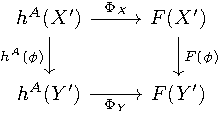
\includegraphics[width=5cm]{./figures/Cat3.pdf}
\caption{此图交换} \label{Cat_fig3}
\end{figure}
即 $F(\phi)(\Phi_{X'}(\psi))=\Phi_{Y'}(h^A(\phi)(\psi))$成立.取 $X'=A,\,Y'=X,\,\phi=f:A\to X,\,\psi=\opn{id}_A:A\to A$,则有 $F(f)(\Phi_A(\opn{id}_A))=\Phi_X(h^A(f)(\opn{id}_A))=\Phi_X(f\circ\opn{id}_A)=\Phi_X(f)$.此时计算 $(n\circ m)(\Phi)$, $m(\Phi)=\Phi_A(\opn{id}_A)=u$, $n(u)=\Psi$,其中 $\Psi_X(f)=F(f)(\Phi_A(\opn{id}_A))$.据前文,有 $\Phi_X(f)=F(f)(\Phi_A(\opn{id}_A))=\Psi_X(f)$,即得 $\Psi=\Phi$.
\end{itemize}
\begin{exercise}{}
模仿上述证明,证明Yoneda引理的第二部分.
\end{exercise}